\section{Threat model}
\label{sec:threat_model}

Three classes of threats to agent workflow safety are considered:

\paragraph{T1: Developer mistakes.}
A developer may inadvertently create a workflow with structural defects:
unreachable exit nodes, dead-end branches that silently drop execution,
routers with incorrectly typed edges, or tool nodes that lack explicit
declarations. Such defects arise naturally from iterative development and
are difficult to catch by manual inspection, especially in large graphs.

\paragraph{T2: Malicious workflow injection.}
An adversary with write access to workflow definitions (e.g., via
compromised configuration files, a shared workflow registry, or a
supply-chain attack on a workflow library) may craft topologies that
bypass safety gates---for example, adding a conditional branch that
routes around a required human-approval node.

\noindent
\emph{Trust assumptions for T2.}
The deployment model assumes an architecture where Agentproof runs as a
mandatory verification gate in a trusted CI/CD pipeline (e.g., a
GitHub Actions workflow or a build system pre-deploy hook).
The adversary can modify workflow definition files (checked into
version control), but \emph{cannot} modify the CI/CD pipeline
configuration, the verification tool, or the extractor
implementation. This is analogous to how static linters catch
malicious code contributions in open-source projects: the linter is
trusted; the contribution is not.

\noindent
\emph{What T2 does not cover.}
An adversary who compromises the build system itself, the Agentproof
binary, or the framework runtime can bypass verification entirely.
Such attacks require integrity protection at the infrastructure level
(code signing, secure boot, access controls) and are outside the scope of this work.

\noindent
\emph{Practical caveat.}
T2 attacks have not yet been observed in the wild against agent workflow
registries. This threat class is included because the attack surface
exists in principle (shared repositories, pip-installable workflow
packages) and because defending against it requires no additional
machinery beyond the structural checks already needed for T1. No
adversarial evaluations have been conducted to determine whether a
sophisticated attacker could craft topologies that evade all six
structural checks while still achieving a malicious objective; such
red-teaming is an important direction for future work.

\paragraph{T3: Runtime graph mutation.}
Some frameworks allow dynamic modification of the workflow graph during
execution (e.g., adding agents to a team, modifying transition rules).
If the post-mutation graph is not re-verified, the guarantees established
at deployment time may no longer hold.

\medskip

\noindent
\textbf{Trust boundary.}
The approach assumes that the framework API semantics (e.g., LangGraph's
\texttt{StateGraph}, CrewAI's \texttt{Crew}) are correct: the extractor
faithfully reads the graph structure that the framework will execute.
The Python runtime and the extractor implementation are within the
trusted computing base. The \emph{workflow definition} authored or
modified by developers and the \emph{LLM outputs} generated at
runtime are \emph{not} trusted.

\medskip

\noindent
\textbf{Scope.}
The structural checks and temporal monitors address threats T1
and T2 statically: they detect defective or malicious topologies before
deployment. Threat T3 requires either runtime re-verification or
immutable workflow definitions; this is discussed in
Section~\ref{sec:limitations}.
LLM output content (e.g., prompt injection, toxic generation) is
explicitly out of scope; this is addressed by complementary runtime
guardrails (Section~\ref{sec:related_work}).

\begin{figure}[t]
\centering
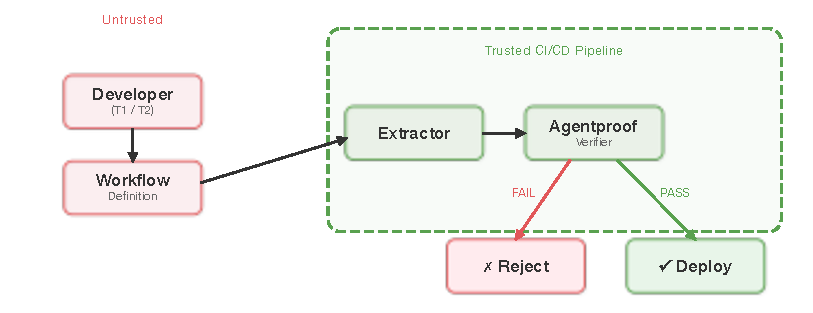
\includegraphics[width=\linewidth]{figures/deployment.pdf}
\caption{Deployment model for T2: Agentproof as a CI/CD verification
gate. The workflow definition is untrusted; the extractor, verifier,
and pipeline are within the trusted computing base.}
\label{fig:deployment}
\end{figure}

\begin{table}[t]
\centering
\small
\caption{Threat classes and Agentproof coverage.}
\label{tab:threats}
\begin{tabular}{@{}llcc@{}}
\toprule
\textbf{Threat} & \textbf{Example} & \textbf{Static} & \textbf{Runtime} \\
\midrule
T1: Dev.\ mistake & Dead-end node & \checkmark &   \\
T1: Dev.\ mistake & Unreachable exit & \checkmark &   \\
T1: Dev.\ mistake & Missing human gate & \checkmark &   \\
T2: Injection & Bypassed approval & \checkmark &   \\
T2: Injection & Added unsafe tool path & \checkmark &   \\
T3: Mutation & Dynamic agent addition & re-verify\textsuperscript{*} & \checkmark \\
  & Toxic LLM output &   & \checkmark \\
\bottomrule
\end{tabular}
\par\smallskip
\raggedright\footnotesize
\textsuperscript{*}Addressed if the graph is re-verified after mutation.
\end{table}
